%% StufungKugelnB

\documentclass[tikz,convert={outfile=\jobname.png}]{standalone}
\usepackage{tikz}


\begin{document}
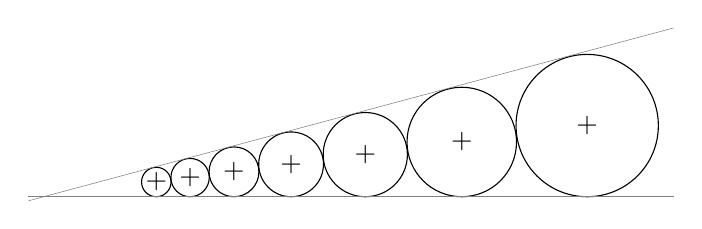
\begin{tikzpicture}

\newcommand{\win}{15};
\newcommand{\start}{1.1}
\newcommand{\sinconst}{1.3} % für winkel = 30 --> 1.698
							% für winkel = 15 --> 1.3
							% für winkel = 60 n--> 3
							
							
							% Vorschrift:
							% (1+sin(\win/2))/(1-sin(\win/2))

\foreach \x [count=\xi] in {1,2,...,7} {

\draw(\start*\sinconst^\x,\start*\sinconst^\x * tan{.5*\win})node {+}circle(\start*\sinconst^\x * tan{.5*\win});
};

\draw[help lines] (-0.2,0)--(8,0);
\draw[help lines] (180+\win:0.2)--(\win:8/cos{\win});


\end{tikzpicture}
\end{document}